% !TEX encoding = UTF-8
% !TEX TS-program = pdflatex
% !TEX root = ../tesi.tex

%**************************************************************
\chapter{Progettazione e codifica}
\label{cap:progettazione-codifica}
%**************************************************************

\vspace{0.5em}
\begin{figure}[!h] 
	\centering 
	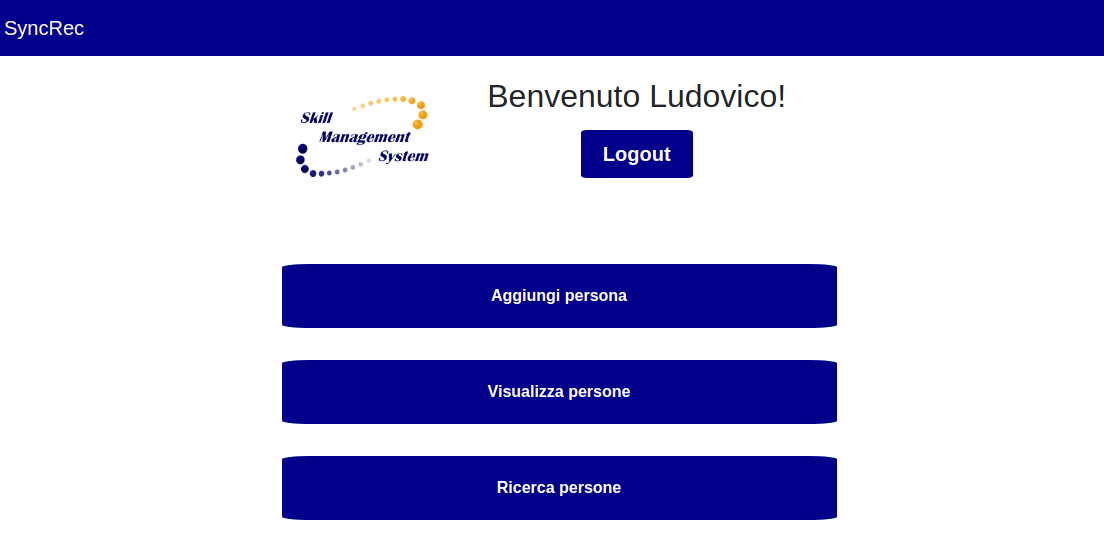
\includegraphics[width=1\columnwidth]{immagini/svil/homepage} 
	\caption{Schermata della homepage}
	\label{figura:homepage}
\end{figure}

\vspace{0.5em}
\begin{figure}[!h] 
	\centering 
	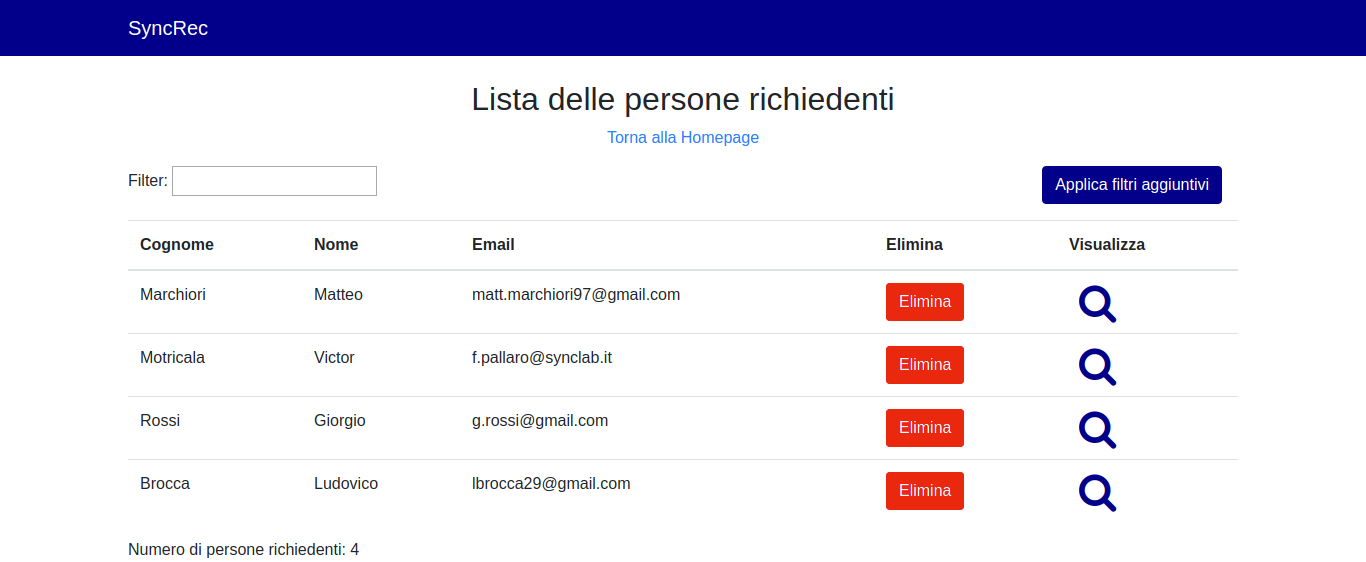
\includegraphics[width=1\columnwidth]{immagini/svil/lista} 
	\caption{Schermata della visualizzazione lista degli applicant}
	\label{figura:lista}
\end{figure}

\vspace{0.5em}
\begin{figure}[!h] 
	\centering 
	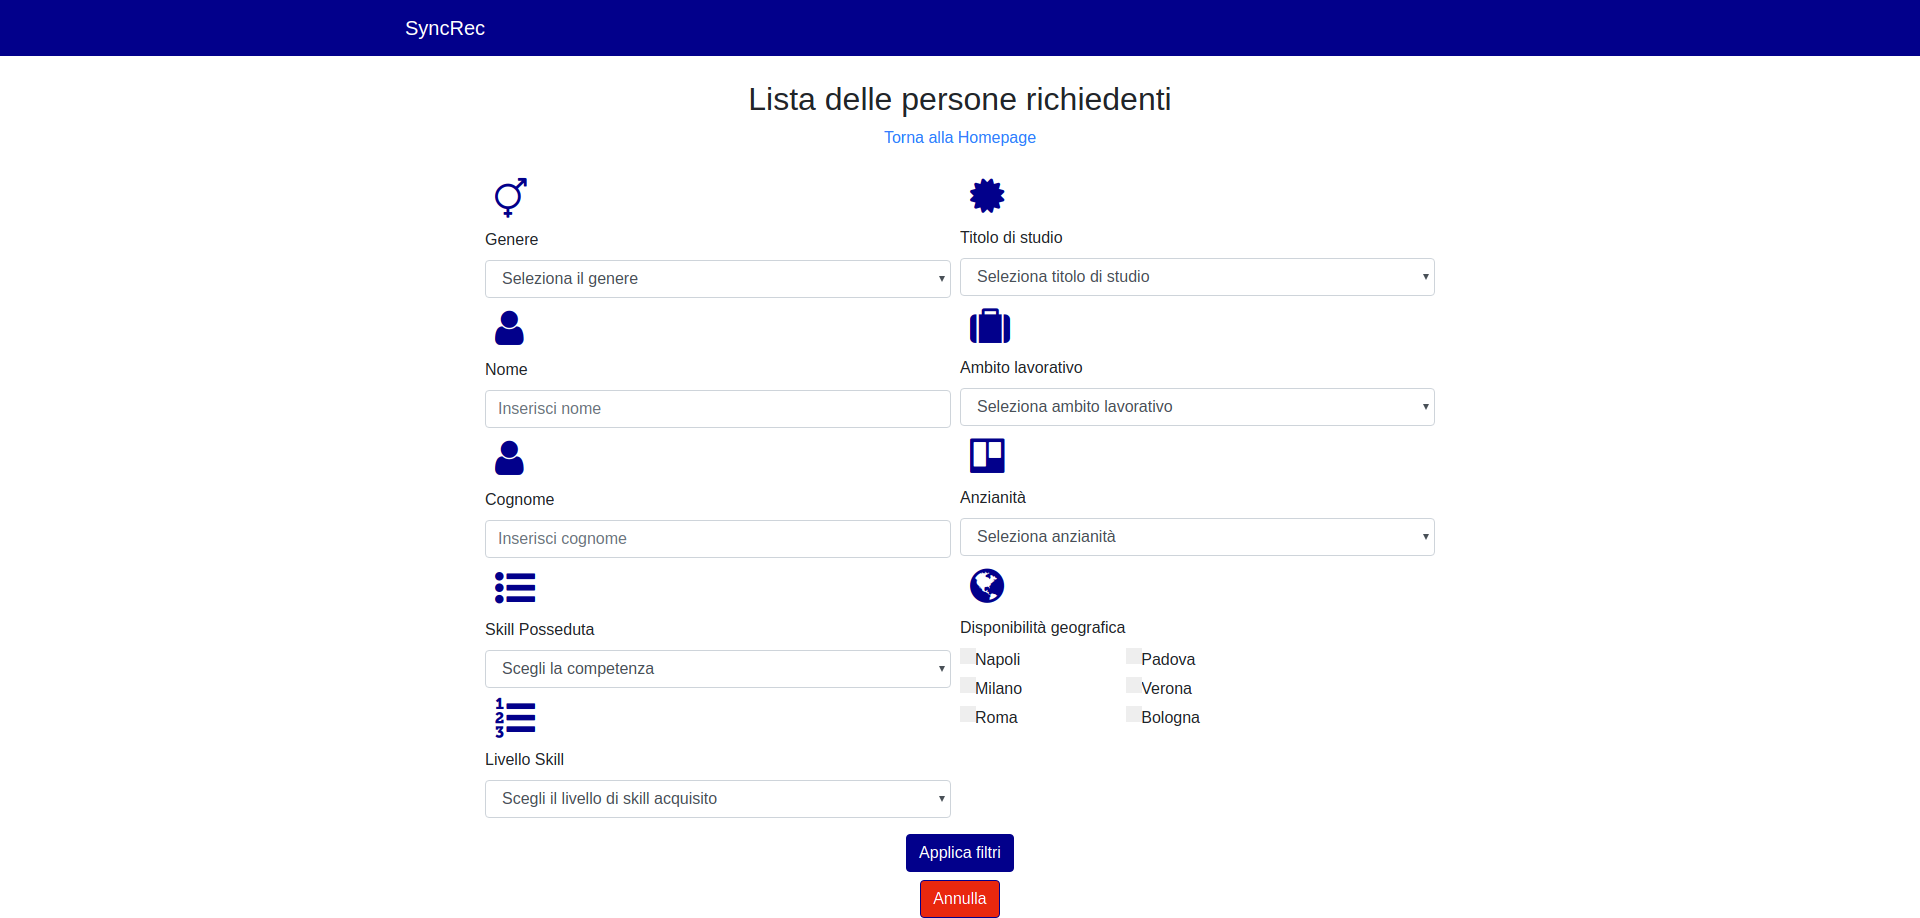
\includegraphics[width=1\columnwidth]{immagini/svil/filtri} 
	\caption{Schermata della selezione dei filtri da applicare alla lista degli applicant}
	\label{figura:filtri}
\end{figure}

\vspace{0.5em}
\begin{figure}[!h] 
	\centering 
	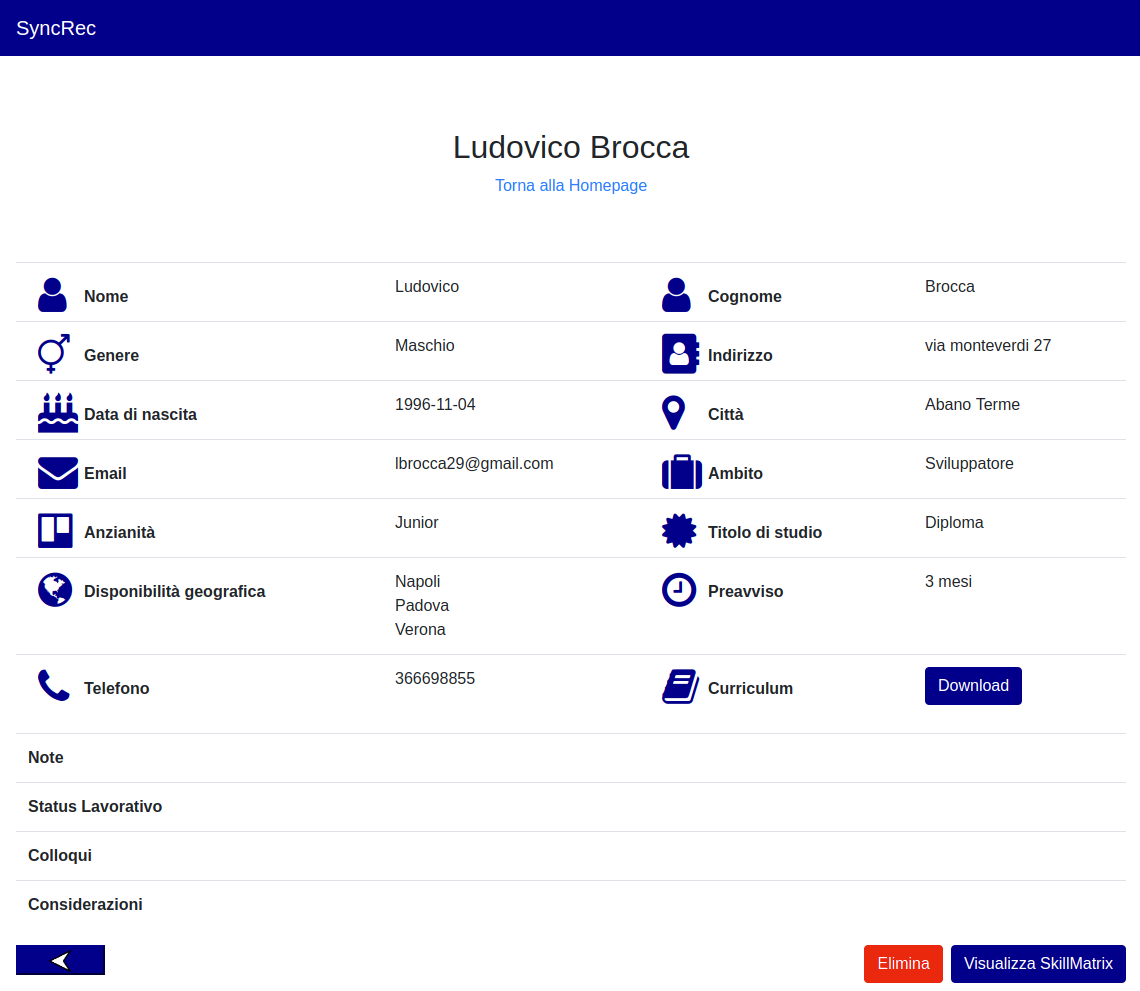
\includegraphics[width=1\columnwidth]{immagini/svil/applicant}
	\caption{Maschera CRUD del singolo applicant}
	\label{figura:applicant}
\end{figure}


\vspace{0.5em}
\begin{figure}[!h] 
	\centering 
	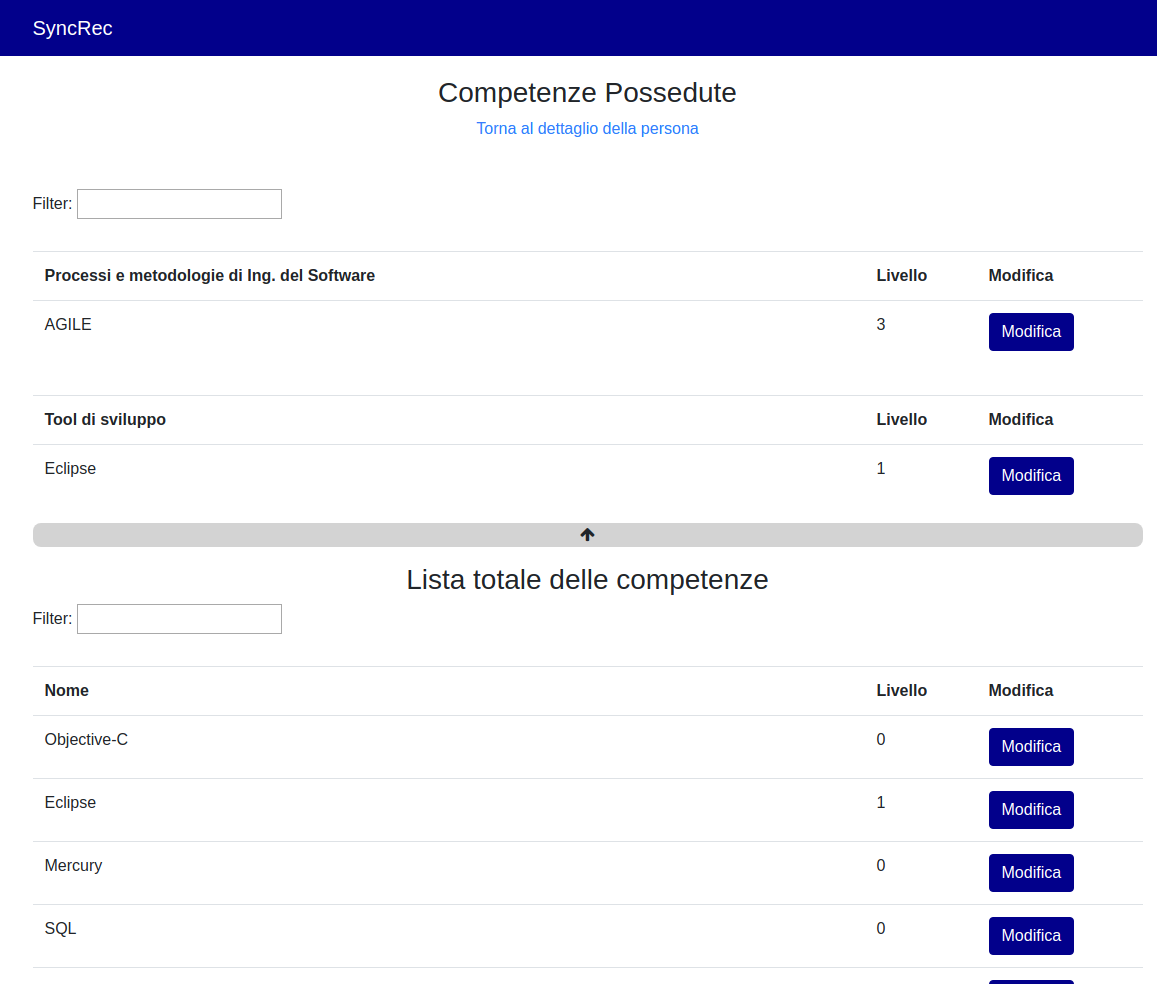
\includegraphics[width=1\columnwidth]{immagini/svil/skillmatrix} 
	\caption{Maschera CRUD dello skillmatrix}
	\label{figura:skillmatrix}
\end{figure}



